lightning\section{Acoustic security}

The second important topic to discuss in this study is the security of rocket and
launch pad itself against the acoustic waves produced by the rocket engines during
launch phase.

Rocket launches generate a significant amount of acoustic energy. The primary
origin of that noise is due to the high jet exhaust velocity required to accelerate
the vehicle during takeoff. Shock waves are created by the collision of ambient air
with the supersonic exhaust plume, and the intensity of the sound waves generated
depends basically on both the size of the rocket and the exhaust
velocity. Typical, the peak noise levels of a launch are around 170-200 dB and are
distributed in the low to midfrequency range, from 2 Hz to 20 kHz. This is
exactly the range where the transmitted energy and power can cause damage to
buildings and humans\cite{2016Teitel}.

\subsection{Rocket Launch Noise Mitigation Techniques}

As in many engineering applications, noise mitigation can be achieved by control
of vibration boundaries and control of unsteady flow phenomenon. This techniques
can be divided in two: active noise control (ANC) and passive noise control (PNC).
The first ones involves using some external power to reduce vibrations in real-time,
and the second is done by introducing devices or materials that actually reduce
the intensity of the sound waves \cite{2017Lubert}.

ANC is typically more feasible and efficient at low frequencies.
However, it is generally hard to achieve in a launch pad environment, where the high frequency
content is particularly intense and is of greatest concern for two reasons. The first is that during
launch, it is enhanced due to both deflected flow noise and ground reflections. Secondly, it
causes a large number of stress reversals (changes from compressional to tensional stress)
in the vehicle, payload, facility..., which can cause fatigue failure during the launch phase
or early flight phase. Thus it is passive
treatments which are more commonly used to mitigate rocket launch noise. Some of the
typical techniques are water injection systems, flame deflection or the proper choice of nozzle configuration.

Water-based acoustic suppression systems are a very common way to do this noise reduction
on launch pads. They use to reduce the noise by 3 to 5dB\cite{2016Pico}. There are two
primary types of water-based acoustic
suppression system; a below-deck system where water is injected into the exhaust plume with
the aim of reducing far-field noise by more rapid dispersion of the rocket exhaust \cite{2014Allgood} or an
above-deck system where water is injected around the pad. Below-deck systems are generally
used to suppress noise during the hold-down phase of the rocket immediately before launch. At
this time, the engines are typically at around 60\% of their full power, just prior to full ignition
and liftoff. Above-deck suppression systems, generally provide a 2-3dB
reduction in sound \cite{2015Houston}. In addition to suppressing the noise, the water also provides cooling to
the launch pad and environs, although care has to be taken not to deluge the pad.
Even water is a very extended way to do this job, an important disadvantage to
this technique is that it can degrade materials and structures\cite{2016Pico}, and
adversely affect the diffuser performance \cite{2014Allgood}.

Figure \ref{fig:deluge_39b_kennedy} shows a test of a water deluge in 39B launch
pad at Kennedy Space Center.

\begin{figure}[h]
	\centering
	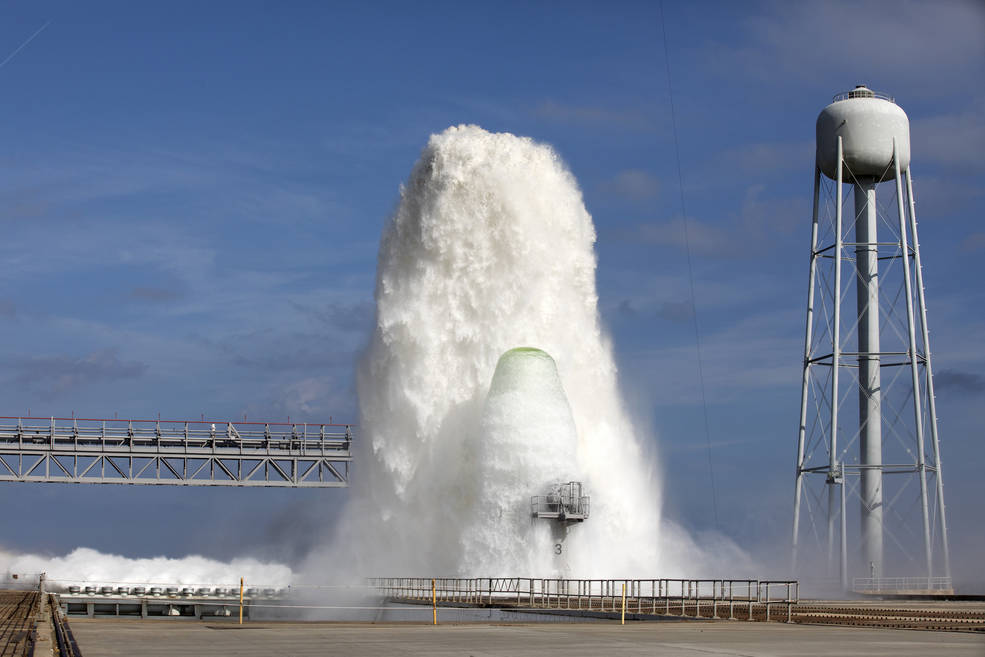
\includegraphics[width=0.8\textwidth]{img/launch_pad_39b_water_deluge_test.jpg}
	\caption[Water deluge system test at Kennedy Space Center]
	{About 450,000 gallons of water flowed at high speed from a holding
	tank through new and modified piping and valves, the flame trench and
	mobile launcher interface risers during a wet flow test at Launch Pad
	39B at NASA's Kennedy Space Center in Florida. Photo credit: NASA/Kim Shiflett}
	\label{fig:deluge_39b_kennedy}
\end{figure}

Also it can be seen in the next picture (figure \ref{fig:fh_launch}) from the
first launch of the Falcon Heavy in launch pad 39A at Kennedy Space Center, the
water deluge system working. Actually it starts working around 10 seconds before
the lift-off at half power. Some seconds before the release of the rocket, the main
engine starts-up at low throttle, and it went max throttle when lift-off. At the
same time, water flow also increases until max flow.

\begin{figure}[h]
	\centering
	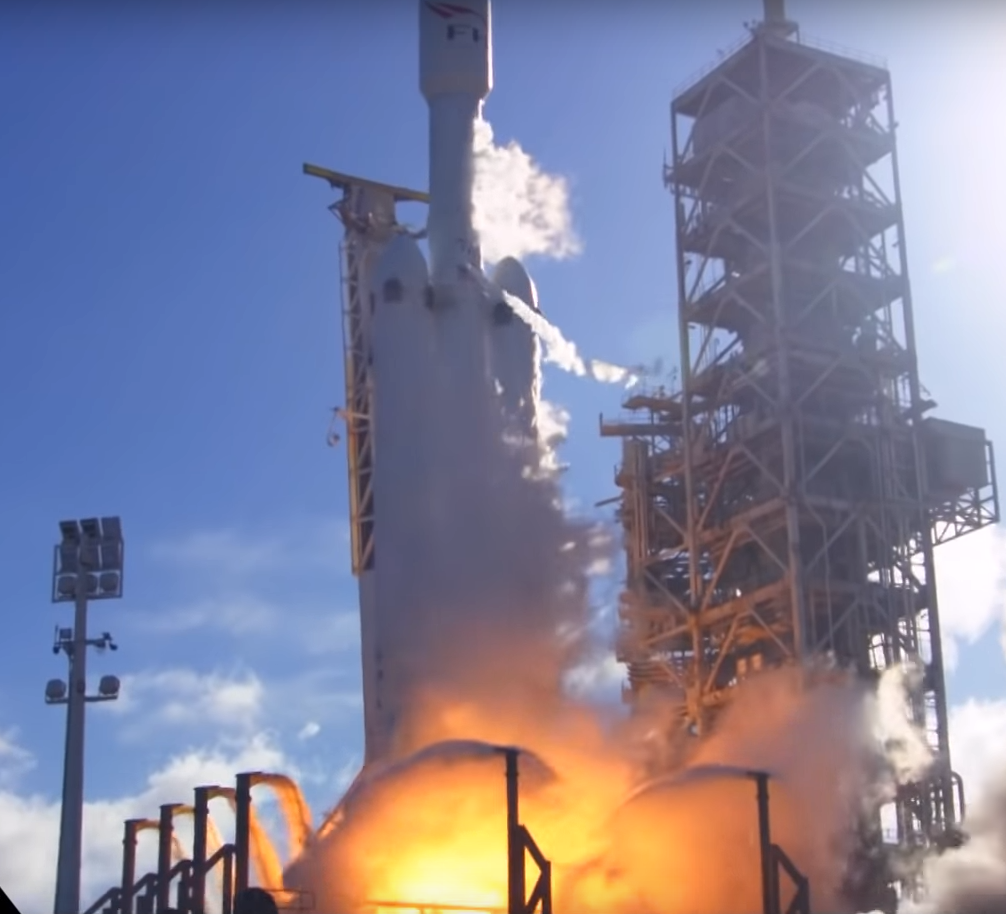
\includegraphics[width=0.8\textwidth]{img/falcon_heavy.png}
	\caption[Falcon Heavy Launch]
	{Water deluge system working during Falcon Heavy launch on launch pad 39A
	at Kennedy Space Center, on 6th of February, 2018. Photo credit: Youtube
	video, Falcon Heavy Test Flight. SpaceX}
	\label{fig:fh_launch}
\end{figure}

\subsection{Design of acostic protection systems}

\subsubsection{Scaled model technique}

As seen in the case of lightning protection, one way to study the acoustic behaviour
of a launch pad is to design a scale model of the building and attack it with sound
waves of different frequencies within the range of the expected real noise.
Some studies \cite{2016Pico} has been developed in this way, for example for the VEGA rocket launch
pad in Kourou (French Guyana), for ESA, which is shown in figure \ref{fig:vega_real}.

\begin{figure}[h]
	\centering
	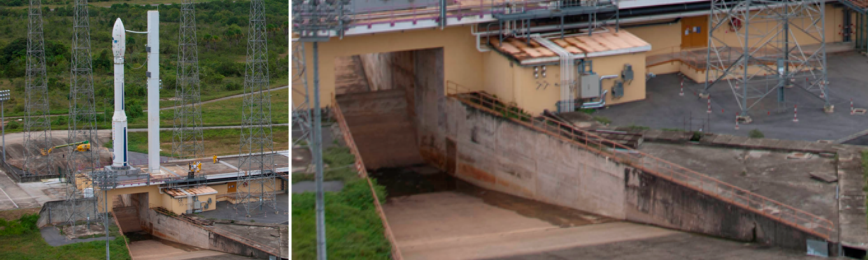
\includegraphics[width=\textwidth]{img/vega_real.png}
	\caption[VEGA launch pad]
	{A picture of the real VEGA launch pad (left), and (right) the detail of
	one of the ducts for flame deflector}
	\label{fig:vega_real}
\end{figure}

After that, it was created a model that is shown in picture \ref{fig:vega_model}.
The model is 1:25 smaller than the real building, and it's built-up with Medium
Density Fiberboard (MDF). The real noise intensity of the VEGA launcher is supposed
to be around 180dB, which is something that can not be simulated in a anechoic chamber
by usual methods, so this test was only to analyse the attenuation of the noise in
different angles and frequencies.

\begin{figure}[h]
	\centering
	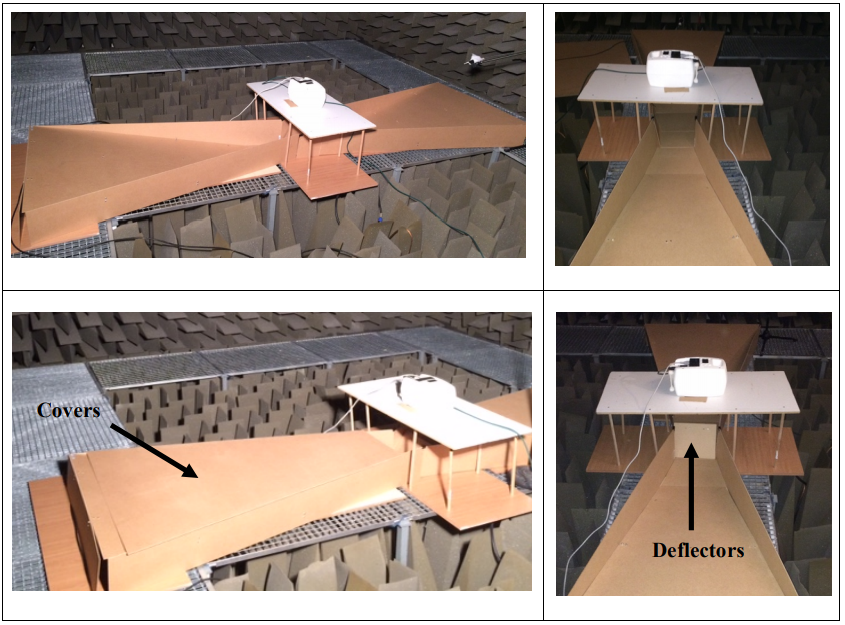
\includegraphics[width=0.8\textwidth]{img/vega_model.png}
	\caption[Scale model of VEGA launch pad for acoustic experiment]
	{Some pictures of the acoustic scale model used for VEGA launch pad}
	\label{fig:vega_model}
\end{figure}

\subsubsection{Numerical methods techniques}

Also, another way to simulate acoustic performance of launch pads is by means of
computational techniques. This techniques are quite advanced today to simulate the
behaviour of sound waves within a gas and could help in the design of better flame
deflectors to reduce dangerous reflections to the rocket.

For example you can create a mesh model for the flame deflector tube, as shown in
the figure \ref{fig:compu_model} from Lubert study,\cite{2017Lubert} and then,
using a computational fluid dynamics method
it can be obtained the resultant shockwave and intensities in different points of the
structure, and it would help in the better design of the building.

\begin{figure}[h]
	\centering
	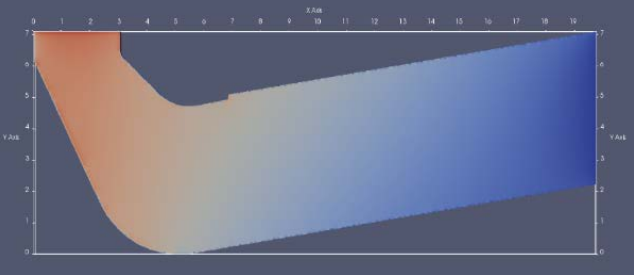
\includegraphics[width=0.6\textwidth]{img/compu_model.png}
	\caption{Computational mesh created for acoustic analysis of launch pad}
	\label{fig:compu_model}
\end{figure}

In figure \ref{fig:compu_results} it's shown the result of that simulation in terms of
air pressure, temperature and velocity, and from that it can be derived pressures
and temperatures on solid surfaces.

\begin{figure}[h]
	\centering
	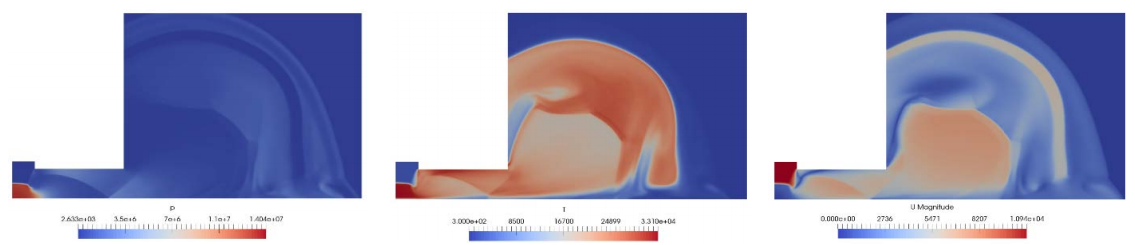
\includegraphics[width=\textwidth]{img/compu_results.png}
	\caption[Results of the computational acoustic simulation]
	{Results of the computational simulation, from left to right: pressure, temperature
	and velocity}
	\label{fig:compu_results}
\end{figure}
